\documentclass{article}
\usepackage{graphicx}
\usepackage[margin=1.5cm]{geometry}
\usepackage{amsmath,amsfonts}

\begin{document}

\title{Tuesday Reading Assessment: Unit 2, Ohm's Law and Batteries, Kirchhoff's Rules}
\author{Prof. Jordan C. Hanson}

\maketitle

\section{Memory Bank}

\begin{itemize}
\item $i_{\rm in} = i_{\rm out}$ ... Kirchhoff's junction rule.
\item $\epsilon_1 + \epsilon_2 + \epsilon_3 + ... = 0$ ... Kirchhoff's loop rule.
\end{itemize}

\section{Kirchhoff's Rules Tutorial}

\begin{enumerate}
\item Recall the Kirchhoff's Rules tutorial video 1.  We solved for the current $i_1$ in Fig. \ref{fig:dura}. (a) What is $i_2$? Once you find $i_2$, find $i_3$ using the junction rule.  What does the sign of $i_3$ tell us about the lower battery? (b) Suppose the emf of battery 2 was raised to $\epsilon_2 = 12$ V, and we observe that $i_1 = 1.2$A and $i_2 = 1.2$A. What is $i_3$?
\begin{figure}[ht]
\centering
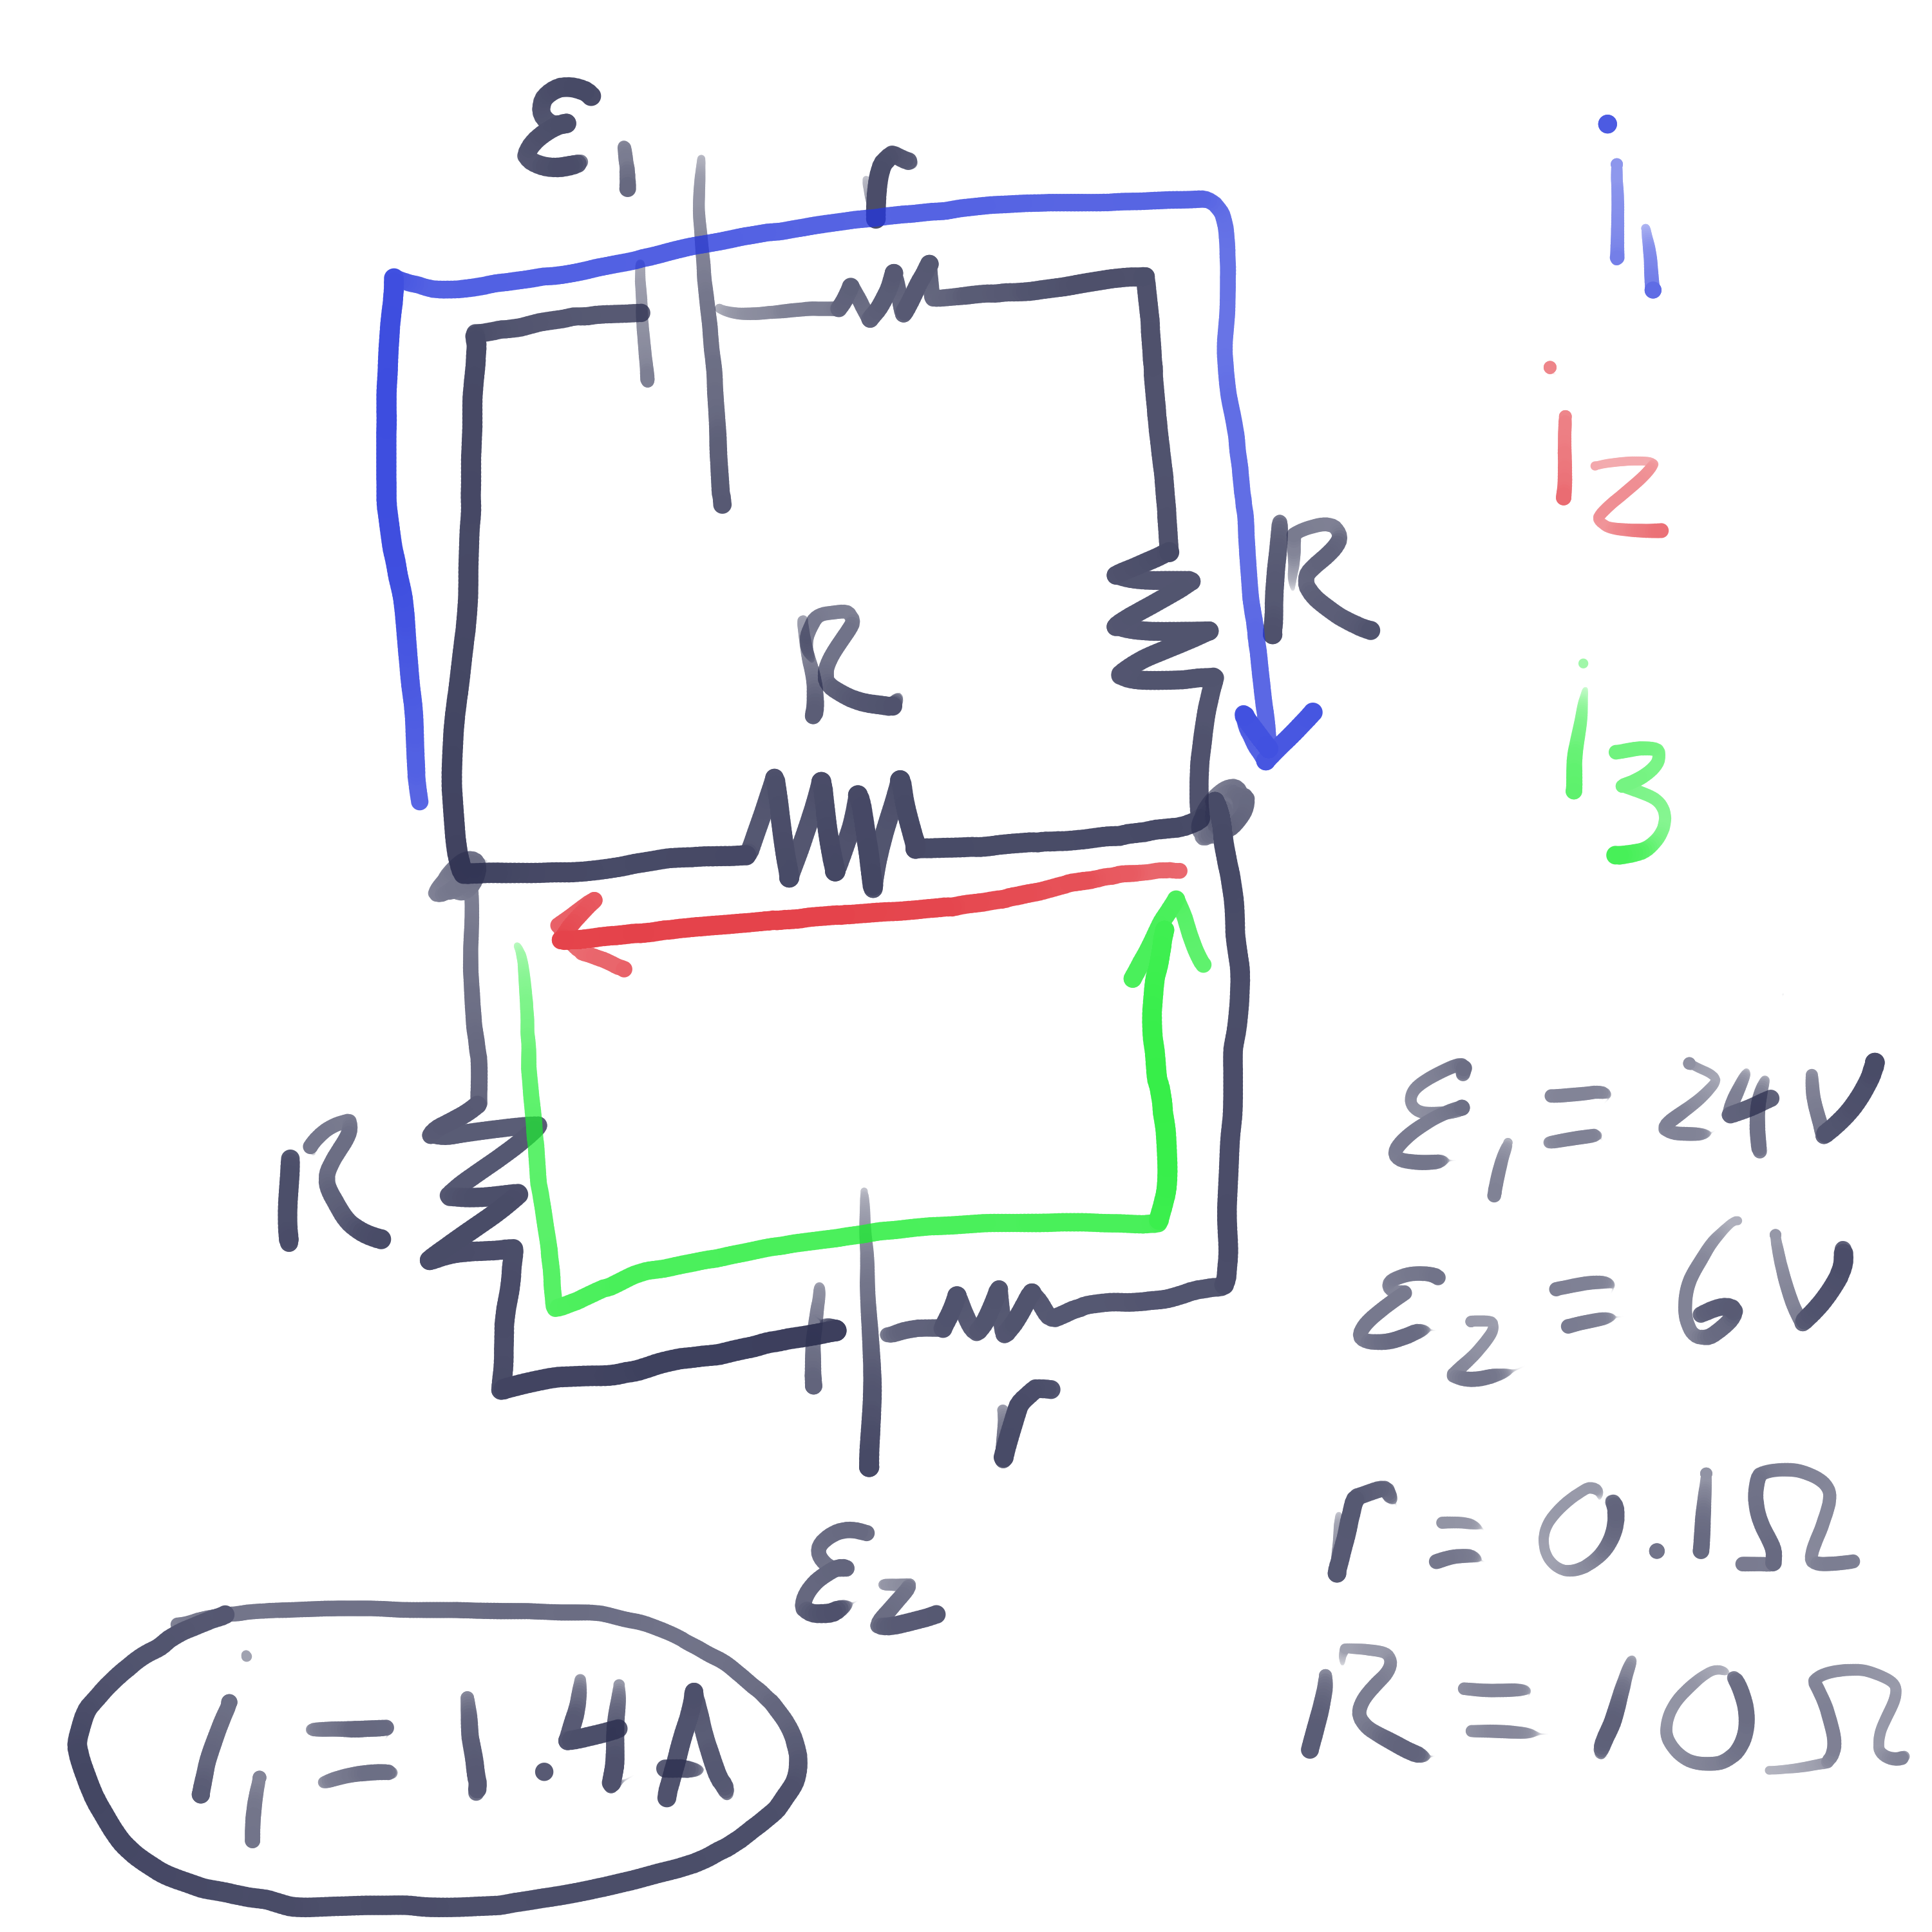
\includegraphics[width=0.4\textwidth]{kirchhoff_tutorial_circuit1.png}
\caption{\label{fig:dura} The circuit from Kirchhoff tutorial video 1.}
\end{figure}
\end{enumerate}

\end{document}
